\chapter{i-vectorの抽出精度向上のための発話区間結合手法}
\label{chapter:prob_method}
i-vectorは発話ができるだけ長いほうが正確に話者の特徴を抽出することができる。そこで、時系列順に並んでいる発話区間のうち、前後の発話が同一話者である可能性が高い発話区間を結合、擬似的に長い発話を作成する。本稿では発話から抽出できるi-vectorに加えて、「発話の時間間隔」「発話環境」を考慮した2通りの手法で発話区間を結合した。図\ref{fig:indexing2}は本稿の提案手法を組み込んだインデックス付与までの流れである。

\begin{figure}[H]
  \begin{center}
    \includegraphics[scale=0.3]{./figure/indexing2.eps}
  \end{center}
  \caption{提案手法を組み込んだインデクシング手法 \label{fig:indexing2}}
\end{figure}

\section{発話の時間間隔を考慮した発話区間の結合手法}
\label{prob1}
同一話者が連続で発話する場合、間をおかずに次の発話を行うことが多い。そのため、発話区間と発話区間の間(非発話区間)が非常に短いとき、高い確率で同一話者の発話が行われていると考えられる。また、インタビューイや中継アナウンサーなど話者が切り替わった場合、ニュースの画面も切り替わるため非発話区間は長くなる。そこで本手法では、発話から抽出されるコサイン類似度が一定値以上を示し、かつ非発話区間が非常に短いとき、同一話者の発話と判別して発話区間を結合する。

\section{発話環境を考慮した発話区間の結合手法}
\label{prob2}
ニュース番組にはスタジオにいるアンカーのほか、台風の状況を中継する中継アナウンサー、騒音の中でインタビューを受けるインタビューイなどが存在する。そこで、アンカーから中継アナウンサー、インタビューイからアンカーなど話者が切り替わった場合、発話環境が変化することに着目した。本稿で使用する音源識別システムはニュース番組音声を「音声」「背景雑音」「音楽」「無音」のいずれかに分類する。そのため、「音声」以外の区間、つまり非発話区間の音源識別結果である「背景雑音」「音楽」「無音」の検出結果が変化した時、発話環境の変化したと識別することができる。そこで本手法では、発話から抽出されるコサイン類似度が一定値以上を示し、かつ発話環境が変化していないとき、同一話者として発話区間を結合する。\par
